%Tipo de documento
\documentclass[12pt,a4paper]{article}

%PAQUETES

%Parsear en .pdf
\usepackage[pdftex]{color,graphicx}

%Castellano
\usepackage[spanish]{babel}
\usepackage[utf8]{inputenc}

%Matematica
\usepackage{amsmath, amssymb, amsfonts}

\begin{document}

\title{Juntura Metal-Semiconductor.}

\author{$\Gamma$}

\maketitle

\section{El diodo de barrera Schottky.}

En esta sección consideraremos las junturas metal-semiconductor rectificantes, o \emph{diodos de barrera Schottky}. En la mayoría de los casos, los contactos rectificantes se hacen sobre semiconductores de tipo n, por esta razón nos concentraremos en este tipo de diodo.

\subsection{Características cualitativas.}

Los diagramas de bandas ideales para un metal y un semiconductor de tipo n, antes de hacer contacto, se muestran en la figura 1. El nivel de vacío se usa como un nivel de referencia (es cuando los electrones son completamente libres).

\begin{figure}[ht!]
\begin{center}
%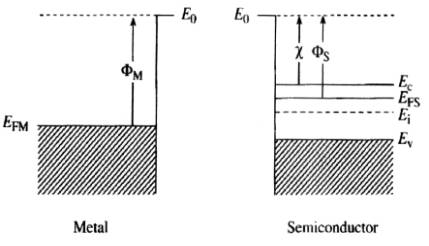
\includegraphics[width=0.7\textwidth]{metalsemiconductorsincontacto.png}
\caption{Diagrama de bandas de un metal y un semiconductor antes de hacer contacto.}
\end{center}
\end{figure}

El parámetro $\phi _{m}$ es la función de trabajo del metal (medida en volts), $\phi _{s}$ es la función de trabajo del semiconductor y $\chi$ es la afinidad electrónica. En la figura 1 asumimos que $\phi _{m}>\phi _{s}$. El diagrama de bandas ideal, en equilibrio térmico, para la juntura metal-semiconductor en esta situación es el que se presenta en la figura 2.

\begin{figure}[ht!]
\begin{center}
%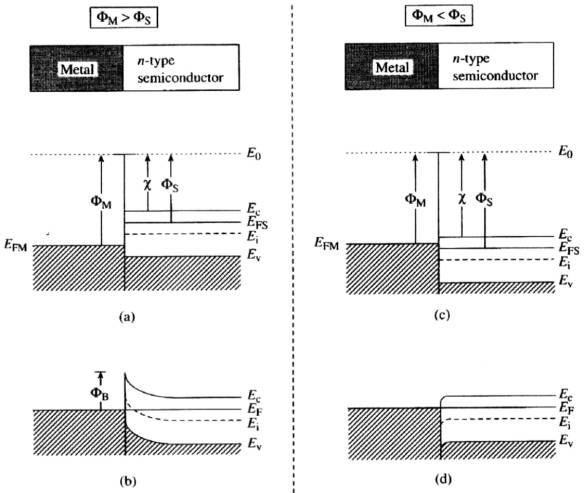
\includegraphics[width=0.7\textwidth]{metalsemiconductorencontacto.png}
\caption{Diagrama de bandas de un metal y un semiconductor al hacer contacto, para el caso en que $\phi _{m}>\phi _{s}$.}
\end{center}
\end{figure}

Antes de hacer contacto, la energía de Fermi en el semiconductor está por encima de la energía de Fermi en el metal. Para que la energía de Fermi se vuelva constante, a través del sistema, en equilibrio térmico, los electrones del semiconductor deben fluir a los estados vacíos del metal (recordar que la energía de Fermi es indicativo de todos los estados ocupados a 0K, entonces, si la energía de Fermi en el semiconductor es mayor, quiere decir que, en el metal, hay estados de energía menor que no han sido ocupados, y como ley fundamental, las partículas ocupan los estados de menor energía, los electrones del semiconductor fluirán hacia el metal). Cuando esto suceda, átomos donores permanecerán en el semiconductor, creando una zona de carga espacial.

El parámetro $\phi _{B_{0}}$ es la altura ideal de la barrera del contacto semiconductor, es la barrera de potencial que ven los electrones del metal al intentar moverse hacia el semiconductor. Esta barrera se conoce como la \emph{barrera de Schottky} y viene dada, idealmente, por
\[ \phi _{B_{0}}=\phi _{m} - \chi \]

En el lado del semiconductor, $V_{bi}$ es la barrera de potencial interna. Esta barrera, similar al caso de la juntura pn, es la barrera que ven los electrones en la banda de conducción del semiconductor, para moverse al metal. La barrera de potencial interna viene dada por
\[ V_{bi}=\phi _{B_{0}} - \phi _{n} \]
lo que hace que $V_{bi}$ sea, en parte, función del dopaje, como en el caso de la juntura pn.

Si aplicamos una tensión positiva al semiconductor respecto del metal, la altura de la barrera semiconductor-a-metal se incrementa, mientras que $\phi _{B_{0}}$ permanece constante en este caso ideal. Esta es la condición de polarización inversa. Si una tensión positiva es aplicada al metal respecto del semiconductor, $V_{bi}$ se reduce mientras que, $\phi _{B_{0}}$ permanece esencialmente constante. En este caso, los electrones pueden fluir fácilmente del semiconductor al metal dado que la barrera se redujo. Esta es la condición de polarización directa. En la figura 3 podemos observar los diagramas de bandas para cada caso, donde $V_{R}$ es la tensión aplicada en polarización inversa y $V_{a}$ es la tensión aplicada en polarización directa.

\begin{figure}[ht!]
\begin{center}
%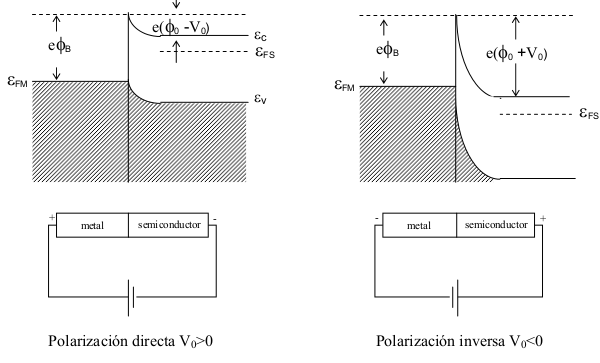
\includegraphics[width=0.95\textwidth]{metalsemiconductorpolarizacion.png},
\caption{Diagrama de bandas de la juntura M-SC en el caso de (a) polarización inversa. (b) polarización directa.}
\end{center}
\end{figure}

Los diagramas de bandas de la figura 3 son bastante parecido a aquellos de la juntura pn. Dada esta similitud, esperaremos que la característica tensión-corriente del diodo de barrera Schottky sea parecida al comportamiento exponencial de la característica del diodo de juntura pn. Sin embargo, en el caso del diodo de barrera Schottky, la corriente se genera por el flujo de los portadores mayoritarios. En polarización directa, la barrera que ven los electrones se reduce, con lo cual estos portadores mayoritarios pueden fluir más fácilmente del semiconductor al metal. Esta corriente de polarización directa va en la dirección del metal al semiconductor (al revés que el movimiento de los electrones), y también es una función exponencial de la tensión de polarización directa, $V_{a}$.

\subsection{Propiedades de la juntura ideal.}

Se pueden determinar las propiedades electrostáticas de la juntura metal-semiconductor (M-SC) de la misma forma que se determinaron para el diodo de juntura pn. El campo eléctrico en la zona espacial de carga viene dado por la ecuación de Poisson
\[ \frac{dE}{dx}=\frac{\rho (x)}{\varepsilon _{s}} \]
donde $\rho (x)$ es la densidad volumétrica de carga y $\varepsilon _{s}$ es la permitividad del semiconductor. Si asumimos que el dopaje del semiconductor es uniforme, entonces, al integrar la ecuación anterior, obtenemos
\[ E= \int \frac{eN_{d}}{\varepsilon _{s}}dx=\frac{eN_{d}x}{\varepsilon _{s}}+C_{1} \]
donde $C_{1}$ es la constante de integración. El campo eléctrico es cero en el borde de la zona de carga espacial, del lado del semiconductor, ($x=x_{n}$ en la figura 3b), con lo cual, la constante de integración es
\[ C_{1}=-\frac{eN_{d}x_{n}}{\varepsilon _{s}} \]
y el campo eléctrico puede ser escrito como
\[ E=-\frac{eN_{d}}{\varepsilon _{s}} (x_{n}-x) \]
que es una función lineal de la distancia, para un semiconductor dopado uniformemente y alcanza un máximo (en módulo) para la interfaz metal-semiconductor. Dado que el campo eléctrico es cero en el interior de un metal, una carga superficial negativa debe existir en el metal, en la interfaz (esto es así porque el campo eléctrico fue originado en los átomos donores de la zona de carga espacial, que son positivos; y como el campo eléctrico nace en carga positiva y muere en carga negativa, debe haber carga negativa en la superficie de la interfaz que haga que el campo eléctrico sea cero dentro del metal).

El ancho de la región de carga espacial, $W$, puede ser calculado como hicimos para la juntura pn. El resultado es idéntico al de una juntura unilateral p$^{+}$n. Para el semiconductor dopado uniformemente, tenemos
\[ W=x_{n}=\bigg( \frac{2 \varepsilon _{s} (V_{bi}+V_{R})}{eN_{d}} \bigg)^{\frac{1}{2}} \]
donde $V_{R}$ es la magnitud de la tensión aplicada en polarización inversa. En este caso, también se utiliza la aproximación de la juntura abrupta.

Se puede determinar, también, una capacitancia de juntura en el mismo modo que se determinó para la juntura pn. Tenemos que
\[ C'=eN_{d} \frac{dx_{n}}{dV_{R}}=\bigg( \frac{e \varepsilon _{s} N_{d}}{2 (V_{bi}+V_{R})} \bigg)^{\frac{1}{2}} \]
donde $C'$ es la capacitancia por unidad de área. Si elevamos al cuadrado la inversa de esta última ecuación, obtenemos
\[ \bigg( \frac{1}{C'} \bigg)^{2}=\frac{2(V_{bi}+V_{R})}{e \varepsilon _{s} N_{d}} \]
Podemos utilizar esta última ecuación para obtener, en una primera aproximación, la barrera de potencial interna, $V_{bi}$, y la pendiente de la curva y encontrar la concentración $N_{d}$. Podemos calcular el potencial $\phi _{n}$ (teniendo la concentración $N_{d}$)\footnote{$\phi _{n}=-\dfrac{kT}{e} \ln \bigg( \dfrac{N_{d}}{n_{i}} \bigg)$ de acuerdo a la sección 3.1 del apunte de juntura pn y diodo. $N_{d}$ es la concentración total de dopantes en el semiconductor.}, y luego determinar el potencial de Schottky, $\phi _{B_{0}}$.

\paragraph{}

\scriptsize No se incluyen efectos no ideales ni función potencial en la juntura. Para función potencial en la juntura recurrir a las diapositivas de Ozols.

\normalsize

\subsection{Relación tensión-corriente.}

La corriente en una juntura M-SC se debe, mayormente, a los portadores mayoritarios de carga, caso contrario a la juntura pn. El proceso básico, en un contacto rectificante con un semiconductor de tipo n, es el transporte de electrones a través de la barrera de potencial, que se puede describir usando la teoría de emisión termoiónica.

Las características de la emisión termoiónica son obtenidas usando las suposiciones de que la altura de la barrera es mucho mayor a $kT$, de tal forma que la aproximación de Maxwell-Boltzmann sea válida y que el equilibrio térmico no se ve afectado por este proceso. En la figura 4 podemos observar una barrera unidimensional con una tensión de polarización directa aplicada, $V_{a}$, y también se pueden observar dos componentes de la densidad de corriente.

\begin{figure}[ht!]
\begin{center}
%\includegraphics[width=0.7\textwidth]{metalsemiconductorconduccion.png},
\caption{Diagrama de bandas para una juntura M-SC en polarización directa.}
\end{center}
\end{figure}

La corriente $J_{s \rightarrow m}$ es la densidad de corriente del electrón debida al flujo de electrones del semiconductor al metal; y la corriente $J_{m \rightarrow s}$ es la densidad de corriente debida a electrones que fluyen del metal al semiconductor. Los subíndices de las densidades de corriente indican la dirección del flujo de electrones. La dirección convencional de corriente es opuesta al flujo de los electrones.

La densidad de corriente $J_{s \rightarrow m}$ es una función de la concentración de electrones que tienen velocidades en dirección $x$ lo suficientemente altas para tener energía capaz de superar la barrera. Podemos escribir
\[ J_{s \rightarrow m}=e \int _{\epsilon'_{c}}^{\infty} v_{x} dn \]
donde $\epsilon'_{c}$ es la energía mínima requerida para la emisión termoiónica hacia el metal, $v_{x}$ es la velocidad de los portadores en la dirección del transporte y $e$ es la magnitud de la carga electrónica. La concentración incremental de electrones viene dada por
\[ dn = g_{c}(\epsilon)f_{F}(\epsilon) d\epsilon \]
donde $g_{c}(\epsilon)$ es la densidad de estados en la banda de conducción y $f_{F}(\epsilon)$ es la función de probabilidad de Fermi-Dirac. Suponiendo que la aproximación de Maxwell-Boltzmann es válida, podemos escribir
\[ dn=\frac{4 \pi (2m^{\ast}_{n})^{\frac{3}{2}}}{h^{3}} \cdot \sqrt{\epsilon - \epsilon _{c}} \cdot e^{-\frac{\epsilon - \epsilon _{F}}{kT}} d\epsilon \]

Si toda la energía de los electrones, superior a $\epsilon _{c}$ la suponemos energía cinéticda, entonces tenemos que
\[ \frac{1}{2} m_{n}^{\ast} v^{2}=\epsilon - \epsilon _{c} \]
La densidad de corriente neta en una juntura M-SC se puede escribir como
\[ J=J_{s \rightarrow m}-J_{m \rightarrow s} \]
que queda definida positiva en la dirección del metal al semiconductor. Encontramos, entonces, que

\[ J=A^{\ast}T^{2}e^{-\frac{e\phi _{B_{0}}}{kT}} (e^{\frac{eV_{a}}{kT}} -1)\]

donde
\[ A^{\ast} \equiv \frac{4 \pi e m_{n}^{\ast} k^{2}}{h^{3}}\]
y este parámetro se llama la constante efectiva de Richardson para la emisión termoiónica.

Esta última ecuación se puede escribir de la forma usual del diodo como
\[ J= J_{sT} (e^{\frac{eV_{a}}{kT}}-1) \]
donde $J_{sT}$ es la densidad de corriente de saturación inversa y viene dada por
\[ J_{sT}=A^{\ast}T^{2}e^{-\frac{e \phi _{B_{0}}}{kT}} \]

\paragraph{}

\scriptsize No incluye la comparación entre el diodo de barrera Schottky y el diodo de juntura pn.

\normalsize

\section{Contactos óhmicos en junturas metal - semiconductor.}

Deben existir contactos entre los dispositivos semiconductores o los circuitos integrados y el mundo exterior. Estos contactos se hacen mediante \emph{contactos óhmicos}. Los contactos óhmicos son junturas M-SC pero que no son rectificantes. Un contacto óhmico es una juntura de baja resistencia que proporciona conducción en ambos sentidos, entre el metal y el semiconductor. Idealmente, la corriente a través del contacto óhmico es una función lineal de la tensión aplicada y la tensión aplicada debe ser muy pequeña. Existen dos tipos de contactos óhmicos posibles: el primero es una barrera ideal no-rectificante, y el segundo es un contacto túnel. Definiremos una resistencia de contacto específica que se usa para caracterizar a los contactos óhmicos.

\subsection{Barreras ideales no-rectificantes.}

En la figura 1 se consideró una juntura M-SC ideal, con un semiconductor de tipo n, y donde $\phi _{m} > \phi _{s}$. La figura 5 muestra la misma juntura ideal, pero para el caso donde $\phi _{m}< \phi _{s}$.

\begin{figure}[ht!]
\begin{center}
%\includegraphics[width=0.9\textwidth]{metalsemiconductorohmica.png},
\caption{Diagrama de bandas para una juntura M-SC tipo n donde $\phi _{m}< \phi _{s}$ (a) Por separado. (b) Juntas.}
\end{center}
\end{figure}

En la figura 5a podemos ver los niveles de energía antes del contacto y, en la figura 5b, la barrera después del contacto, en equilibrio térmico. Para conseguir equilibrio térmico en esta juntura, los electrones fluirán desde el metal a los estados de menor energía, libres en el semiconductor, lo que hace que la superficie del semiconductor sea más de tipo n. Este exceso de electrones en el semiconductor de tipo n existe, esencialmente, como una densidad de carga superficial. Si una tensión positiva es aplicada al metal, respecto del semiconductor, no existe ninguna barrera para los electrones que fluyen del semiconductor al metal. Si una tensión positiva es aplicada al semiconductor, respecto del metal, la altura de la barrera efectiva para los electrones fluyendo del metal al semiconductor será, aproximadamente, $\phi _{B_{0}}=\phi _{n}$, que es considerablemente pequeña para un semiconductor altamente dopado. Para esta polarización, los electrones puede fluir fácilmente del metal al semiconductor.

\begin{figure}[ht!]
\begin{center}
%\includegraphics[width=0.9\textwidth]{ohmicatipop.png},
\caption{Diagrama de bandas para una juntura M-SC tipo p donde $\phi _{m}> \phi _{s}$ (a) Por separado. (b) Juntas.}
\end{center}
\end{figure}

En la figura 6 tenemos una juntura ideal no-rectificante entre un metal y un semiconductor de tipo p. La figura 6a muestra los niveles de energía antes del contacto para el caso donde $\phi _{m}> \phi _{s}$. Cuando se realiza el contacto, los electrones del semiconductor fluirán en el metal para alcanzar el equilibrio térmico, dejando atrás mayor cantidad de estados vacíos o huecos. El exceso en la concentración de huecos hará que la superficie del semiconductor sea más tipo p. Los electrones del metal se pueden mover fácilmente a los estados vacíos en el semiconductor. Este movimiento de carga corresponde a huecos fluyendo del semiconductor al metal.

\subsection{Contacto túnel.}

El ancho de la zona de carga espacial en una juntura M-SC rectificante es inversamente proporcional a la raíz cuadrada del dopaje del semiconductor. El ancho de la zona de vaciamiento disminuye a medida que aumenta la concentración de dopantes en el semiconductor; por lo tanto, como la concentración de dopantes aumenta, la probabilidad de tunelamiento a través de la barrera aumenta.

La corriente de tunelamiento tiene la forma
\[ J_{t} \propto e^{-\frac{e \phi _{B_{0}}}{E_{oo}}} \]
donde
\[ E_{oo}=\frac{e \hbar}{2} \sqrt{\frac{N_{d}}{\varepsilon _{s} m_{n}^{\ast}}} \]
El tunelamiento aumenta exponencialmente con la concentración de dopantes.

\subsection{Resistencia específica de contacto.}

Una figura de mérito de los contactos óhmicos es la resistencia específica de contacto, $R_{c}$. Este parámetro es definido como el inverso de la derivada de la densidad de corriente respecto de la tensión evaluada cuando no hay polarización. Es decir,
\[ R_{c} = \bigg( \frac{\partial J}{\partial V} \bigg)^{-1} \rfloor_{V=0} \qquad [R_{c}]=\Omega-\textrm{cm}^{2} \]
Lo ideal es que $R_{c}$ sea lo más pequeño posible para un contacto óhmico.

Para un contacto rectificante con una concentración moderadamente pequeña de dopantes, la relación tensión-corriente viene dada por la ecuación
\[ J=A^{\ast}T^{2}e^{-\frac{e\phi _{B_{0}}}{kT}} (e^{\frac{eV_{a}}{kT}} -1)\]
La corriente por emisión termoiónica es dominante en estas junturas. En este caso, la resistencia específica de contacto es
\[ R_{c}=\frac{\bigg( \dfrac{kT}{e} \bigg) e^{\frac{e \phi _{B_{0}}}{kT}}}{A^{\ast}T^{2}} \]
La resistencia específica de contacto disminuye rápidamente a medida que disminuye la altura de la barrera.

Para una juntura M-SC con una gran concentración de dopantes, los procesos de tuneleo dominan. Utilizando la ecuación de $J_{t}$ obtenemos
\[ R_{c} \propto e^{\frac{2\sqrt{\varepsilon_{s}m^{\ast}_{n}}}{\hbar} \cdot \frac{\phi _{B_{0}}}{\sqrt{N_{d}}}} \]
que muestra que la resistencia específica de contacto depende fuertemente del dopaje del semiconductor.

La teoría para formar contactos óhmicos es bastante sencilla. Para obtener un buen contacto óhmico, necesitamos crear una barrera pequeña y usar un semiconductor altamente dopado en la superficie. Sin embargo, la tecnología actual para fabricar contactos óhimcos buenos y confiables, no es tan sencilla en la práctica como en la teoría. También resulta más difícil fabricar buenos contactos óhmicos en materiales que tienen un gran ancho de banda. En general, las barreras no son pequeñas en este tipo de materiales y, por lo tanto, deben usarse semiconductores altamente dopados en la superficie para formar un contacto túnel.

\end{document}
